% !TEX root = CSL 2021.tex

%\subparagraph*{Measuring sensitivity and similarity of programs in a compositional way}
In program semantics one is usually interested in capturing notions of behavioral equivalence between programs. However,  
%\textit{i.e.} to describe when two programs behave in the same way, so that replacing one by the other in any context produces no observable change in the result. However, 
in several fields like approximate \cite{Mittal2016}, incremental \cite{Cai2014, Picallo2019} and probabilistic \cite{10.1109/LICS.2015.64} computation, it is often more useful to be able to describe \emph{to which extent}  two programs behave in a similar, although non equivalent way, so that one can measure the change in the result produced by
replacing one program by the other one.
% produces a change in the result which can be quantified and bounded in some way.



This idea has motivated much literature on program (pseudo)metrics \cite{ARNOLD1980181, VANBREUGEL20011,Azevedo_de_Amorim_2017, Escardo1999, BAIER1994171,10.1109/LICS.2015.64, 10.1007/978-3-662-44584-6_4, 10.1007/978-3-662-54434-1_13, 10.1145/3209108.3209149}, that is, on semantics in which types are endowed with a notion of distance measuring the differences in their behaviors. This approach has found widespread applications, for example in differential privacy \cite{10.1145/1932681.1863568, 10.1007/978-3-642-29420-4_3, Barthe_2012}, where one is interested in measuring the \emph{sensitivity} of a program, \textit{i.e.} its capacity to amplify changes in its inputs, and in the study of probabilistic processes \cite{DESHARNAIS2004323, VANBREUGEL2005115, 10.1007/978-3-662-44584-6_4,10.1007/3-540-48224-5_35}.
%
%A similar concern is found in fields like differential privacy \cite{10.1145/1932681.1863568, 10.1007/978-3-642-29420-4_3, Barthe_2012}, where one looks for means to measure the \emph{sensitivity} of a program, that is, of how much a change in the input will affect changes in the output.

 
% More generally, in many situations one wishes to replace some computationally intensive piece of program by a more efficient, although not equivalent, one: t
 
 
% 
%  For example, in the case of the transformation of $\lambda x.\sin(x)$ into $\lambda x.x$, 
% a natural candidate for their ``difference''  would be a function associating a real number $r$, or, say, a closed ball $B$ around $r$, with the \emph{distance} between $\sin(r)$ and $r$ (or with the sup of the distances computed on the points of $B$). 
% 
    
  
%  A  common ground for these approaches is the idea that  of taking program differences as themselves some kind of programs, relating potential errors in input with errors in  output. 

 
  
% 
%  
%% For this reasons, in such frameworks we find two different classes of programs (with different typing structure): \emph{exact} programs, leading from well-defined inputs to well-defined outputs, and \emph{approximate} programs, leading from errors in the input into errors in the output.
%
%
% 
% In this paper we propose a framework to reason about program differences in a contextual way using some kind 
% 
%  

Some recent literature \cite{chaudhuri, dallago:differential-stlc} has highlighted the importance of \emph{contextuality} to reason about program similarity: many common situations  require to measure the error produced by a transformation of the form $\mathtt C[t] \leadsto \mathtt C[u]$, which replaces a program $t$ by $u$ \emph{within a context} $\mathtt C[\ ]$, from a measure of the mismatch between $t$ and $u$ and of the sensitivity of the context $\mathtt C[\ ]$ itself.
 %one looks for ways to measure the similarity between two programs in a \emph{contextual} way: one seeks a bound for the error of replacing a program $t$ by $u$ within a given context
%
%
% between two programs $\mathtt C[t], \mathtt C[u]$, from a measure of the similarity between $t$ and $u$ and, possibly, of the sensitivity of the context $\mathtt C[\ ]$ itself.  
%
%
%the program similarity
%
 %A fundamental aspect to take into account when reasoning about
% The notion of program similarity that these frameworks  
%  is that this notion is highly \emph{contextual}. 
  For instance, the replacement of the program $\lambda x.\sin(x)$ by the identity function $\lambda x.x$
  produces an error whose measure depends on whether
$\lambda x.\sin(x)$
occurs in a context in which it is applied to values close to $0$.
 Similar cases of contextual reasoning can be found  in many areas of computer science. For instance, 
 in numerical analysis (\emph{e.g.}~the Gauss-Newton method) in which a 
 computationally intensive function is replaced by its Taylor's expansion {around some given point}, or in {approximate computing} techniques like \emph{loop perforation} \cite{loopperf}, in which a compiler can be asked to skip a certain number of iterations.% provided this won't exceed some error bound.
 

%, replacing $f$ will not produce a considerable error. However, this transformation would no longer be justified if $f$ were applied on values far from 0.
%Similarly, 
%   one 
% 
% 
% modifies the execution of a loop iterating a given list of instructions and 
% 
%  within a larger program.
 
\subparagraph*{The problem of coupling program metrics and higher-order types}



\begin{figure}
\begin{subfigure}{0.48\textwidth}
\parbox[h][3.5cm][c]{\textwidth}{
\adjustbox{center}{$
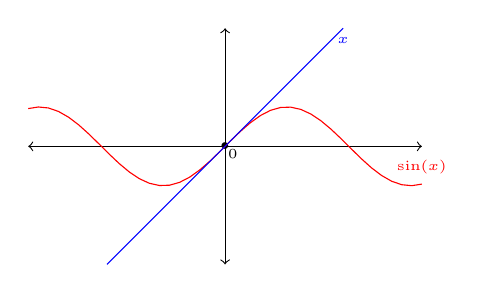
\begin{tikzpicture}[domain=-5:5, scale=0.5]
%\draw[very thin,color=gray] (-0.1,-1.1) grid (3.9,3.9);
\draw[<->]   (-5,0) -- (5,0);
\draw[<->] (0,-3) -- (0,3); % node[above] {$f(x)$};

   \node at (0.2,-0.2){\tiny$0$};
      \node at (0,0){\tiny$\bullet$};

%
\draw[color=red, domain=-5:5, samples=40] plot (\x, {sin(\x r)} ) node[above] {\tiny$\sin(x)$};

\draw[color=blue, domain=-3:3, samples=40] plot (\x,{\x  } ) node[below] {\tiny$x$};


\end{tikzpicture}$}
}
\caption{\small $\sin(x)$ and $x$ are very close around 0, but their distance diverges at $\pm \infty$.}
\label{fig:sinid1}
\end{subfigure} \ \ \ 
\begin{subfigure}{0.48\textwidth}
\parbox[h][3.5cm][c]{\textwidth}{
\adjustbox{center}{$
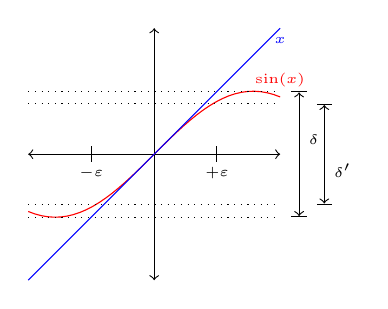
\begin{tikzpicture}[domain=-2:2, scale=0.8]
%\draw[very thin,color=gray] (-0.1,-1.1) grid (3.9,3.9);
\draw[<->]   (-2,0) -- (2,0);
\draw[<->] (0,-2) -- (0,2); % node[above] {$f(x)$};


\draw[|-|] (-1,0) -- (1,0);
\node(r) at (-1,-0.3) {\tiny$-\varepsilon$};
\node(r) at (1,-0.3) {\tiny$+\varepsilon$};
   % \node at (0,0)[circle,fill,inner sep=1pt]{};
%
\draw[color=red, domain=-2:2, samples=40] plot (\x, {sin(\x r) } ) node[above] {\tiny$\sin(x)$};

\draw[color=blue, domain=-2:2,samples=40] plot (\x,{\x  } ) node[below] {\tiny$x$};


\draw[dotted] (-2,1) -- (2,1);
\draw[dotted] (-2,-1) -- (2,-1);

\draw[dotted] (-2,0.8) -- (2,0.8);
\draw[dotted] (-2,-0.8) -- (2,-0.8);

\draw[|<->|] (2.3,1) -- node[above right]{\tiny$\delta$} (2.3,-1);
\draw[|<->|] (2.7,0.8) -- node[below right]{\tiny$\delta'$} (2.7,-0.8);


\end{tikzpicture}$}
}
\caption{\small The self-distances $\delta,\delta'$ of $\sin(x)$ and $x$ in a small interval $[-\varepsilon,\varepsilon]$ of $0$ are very close.}
\label{fig:sinid2}
\end{subfigure}
\caption{The sup-distance is inadequate for contextual transformations.}
\label{fig:sinid}
\end{figure}
 
  While several frameworks  have been developed for contextual reasoning \cite{10.1145/1932681.1863568,Gaboardi_2013,Azevedo_de_Amorim_2017,chaudhuri, dallago:differential-stlc},  these approaches seem to suggest that lifting an account of program
differences in terms of program metrics to a fully higher-order language still constitutes a major challenge. 
%Yet, in this paper we propose a framework which accommodates both aspects.
%
% The question that motivates this paper is whether a notion of program difference of this kind can itself be seen as a metric over the programs of a programming language with higher-order types.  
Suppose to start from a language  containing a type $\mathsf{Real}$ for real numbers on which errors are measured with the standard metric. It is not clear, then, how to lift this metric to higher-order types, \emph{e.g.}~to $\mathsf{Real}\to \mathsf{Real}$, so that distances are measured in a contextual way.



A standard solution is to take the sup-distance, that is, to let, for $f,g:\mathsf{Real}\to \mathsf{Real}$, $d(f,g)=\sup\{d(f(r),g(r))\mid r\in \mathsf{Real}\}$. This solution works well in models in which programs are interpreted as \emph{non-expansive} or \emph{Lipschitz-continuous} maps \cite{Hofmann2014, Azevedo_de_Amorim_2017}. However, as is well-known, such models are not \emph{cartesian-closed}\footnote{In fact, cartesian closed categories of metric spaces and non-expansive functions \emph{do} exist \cite{Escardo1999, Stubbe2009}, but, to our knowledge, none of these categories contains the real numbers with the standard metric.}, so they do not account for 
 the simply-typed lambda-calculus in its full generality, but only for linear or sub-exponential variations of it (such as $\mathsf{Fuzz}$ \cite{10.1145/1932681.1863568,Gaboardi_2013,Azevedo_de_Amorim_2017}).
 Also, it has been shown \cite{10.1109/LICS.2015.64} that in a probabilistic setting the non-linearity of higher-order programs has the effect of \emph{trivialising} metrics, that is, of forcing distances to be either 0 or 1, hence collapsing program distances onto usual notions of program equivalence.
Most importantly, even if one restricts to a sub-exponential language, the sup-distance seems inadequate to account for contextual transformations as the replacement of $\lambda x.\sin(x)$ by $\lambda x.x$ around 0,  as the sup-distance between such programs is infinite (see Fig. \ref{fig:sinid}). 
 
 
On the other side of the coin, other approaches like \cite{chaudhuri, dallago:differential-stlc} are fully contextual and higher-order, but provide, at best, only weak approximations of a standard notion of metric.  
 Nonetheless, these approaches introduce the idea, that we retain here, that program differences must be taken as being themselves some kind of programs, relating errors in input with errors in  output,  and separate programs accordingly in two different classes: \emph{exact} programs, computing mappings from well-defined inputs to well-defined outputs, and \emph{approximate} programs, computing mappings from errors in the input to errors in the output.
%

%
%way to lift a metric $d$ on a set $A$ to a set of functions from $B$ to $A$ is by letting the distance between  be defined as the sup of the distances $d(f(x),f(x))$, with $x$ ranging on $B$.
%This approach is at work in several frameworks
%
%
%A standard way to measure differences between programs is by means of program metrics, that is, by endowing types $A$ with a distance $d:A\times A\to \mathbb R^{+}$. However, program metrics usually fail our compositional demand. Typically, in such models the distance between two programs $f,g: \mathsf{Real}\to \mathsf{Real}$ is computed as the $\sup$ of the distances between the values $f(r)$ and $g(r)$, for $r$ a ground element of $\mathsf{Real}$. 
%This approach is then not fine enough to capture differences which might depend on the context. For instance, whenever $g$ is obtained from $f$ by a truncated Taylor expansion around a point $r$, or by the replacement of a  $\mathsf{while}$ loop in $f$ by its perforation, the $\sup$-distance between $f$ and $g$ will most likely be infinite.
%
%
%A second issue with program metrics is that devising models of higher-order programming languages in which types are metric spaces still remains a non-trivial task. In fact, it is well-known that usual categories of metric spaces (\textit{e.g.} those generated by \emph{Lipschitz-continuous} functions)
%%\footnote{An exception is the metric model of PCF in \cite{Escardo1999}, based on a cartesian closed category of \emph{ultrametric spaces}, which in particular excludes $\R$.} \cite{Hofmann2014}) 
%are not \emph{cartesian-closed}, that is, do not provide models of the simply-typed lambda-calculus, but only of linear or sub-exponential variations of it (such as the system $\mathsf{Fuzz}$ \cite{10.1145/1932681.1863568,Gaboardi_2013,Azevedo_de_Amorim_2017}).
%
%
%; 


%second, such models are not at first sight compatible with the compositional approach advocated above: in a metric model the distance between two functional program is a real number (e.g. the max of the distances between the inputs), and this hardly provides a good compositional notion of difference [EXAMPLE HERE, e.g. sin/id, highlight the role of context, you can't justify contextual transformations].

%EXAMPLE: Newton's approximation works well around some point (so it is contextual) -- see Di Cosmo Tweet on Apollo 11






\subparagraph*{Diameter Spaces}



In this paper we introduce a class of higher-order denotational models, that we call \emph{diameter space models}, to reason about program similarity and approximate program transformations.
In such models a higher-order type $A$ is interpreted as a 4-tuple $(|A|, \intervals{A}, \distances{A}, \diam_{A})$ called a \emph{diameter space}, where $|A|$ is a set of \emph{exact} values, $\intervals{A}\subset \mathcal P(|A|)$ is a complete lattice of \emph{approximate} values, $\distances{A}$ is a \emph{quantale}, and $\diam_{A}: \intervals{A}\to \distances{A}$ is a function, called \emph{diameter}, which provides a quantitative measure of approximate values.





The maps $\diam_{A}$ take their name from the fact that they  
 generalize some properties of the diameter function of the standard metrics on real numbers, in particular, 
the fact that the diameter is \emph{modular} over intersecting intervals (see Fig. \ref{fig:modular}).
Moreover, just like the standard metric on $\mathbb R$ can be recovered from the diameter by $d(x,y)=\mathsf{diam}([x,y])$, the function $\diam_{A}$ induces a \emph{generalized partial metric} $d_{A}:|A|\times |A|\to \distances{A}$ by letting $d_{A}(x,y)=\diam_{A}(x\vee y)$. 


Generalized partial metric spaces (henceforth GPMS) are a well-investigated class of metric spaces that has been widely applied in program semantics \cite{bkmp:partial-metrics, Bukatin1997, doi:10.1111/j.1749-6632.1994.tb44144.x, Schellekens2004, Samet:2013aa, Stubbe2018, HE201999}. 
Such spaces generalize standard metric spaces in that distances
need not be real numbers, but can be functions or any other type of object that leaves in a suitable \emph{quantale} \cite{Hofmann2014}, and \emph{self-distances} $d(x,x)$ need not be $0$ (which in turn leads to strengthen the usual triangular inequality as $d(x,y) + d(z,z)\leq d(x,z)+d(z,y)$).
%\footnote{The adjective ``partial'' comes from the fact that in partial metric semantics like \cite{} the  programs with a non-zero self-distance are those which are not total, in the sense of Scott domains. This will not be the case in our framework. 
%}   
%Observe that not only any standard metric space is a GPMS, but from from any partial metric $d$ one can retrieve a (generalized) metric $d'$ by letting $d'(x,y)=2d(x,y)-d(x,x)-d(y,y)$.


\begin{figure}
\adjustbox{center}{
\begin{tikzpicture}


\draw[|<->|, orange] (-2,0) to node[above] {$a$} (2,0);
\draw[|<->|, blue] (1,0) to node[above]  {$b$} (4,0);
\draw[violet] (1,0) to (2,0);

\draw[|<->|, dashed] (-2,0.8) to node[above] {\tiny$\delta(a\cup b)$} (4,0.8);
\draw[|<->|, dashed] (1,0.5) to node[below] {\tiny$\delta(a\cap b)$} (2,0.5);
\draw[|<->|, dashed] (-2,-0.5) to node[below] {\tiny$\delta(a)$} (2,-0.5);
\draw[|<->|, dashed] (1,-0.8) to node[below] {\tiny$\delta(b)$} (4,-0.8);



\end{tikzpicture}}
\caption{\small The diameter function is \emph{modular} over intersecting real intervals: 
$\mathsf{diam}(a\cup  b)+\mathsf{diam}(a\cap b)=\mathsf{diam}(a)+\mathsf{diam}(b)$ for all $a,b\in [\R]$ such that $a\cap b\neq \emptyset$.
This property is at the heart of our generalization of diameters.}
\label{fig:modular}
\end{figure}


%
%
%In this paper we show that the standard metric on real numbers can be lifted to higher-order types in a novel way, yielding a metric semantics of the simply typed lambda-calculus in which types are interpreted as quantale-valued partial metric spaces. Noticeably, the distances between objects of higher-types are elements of functionals, thus non-numerical, quantales,. This on the one hand allows us to faithfully model arbitrary functions, thus deviating from classic metric semantics, and on the other enables contextual reasoning. 
%
%%The partial metrics induced by diameter spaces 
%% generalize some properties of the standard metric on real numbers: the fact that the distance between two points $x,y$ coincides with the diameter of the smallest \emph{interval} containing them, 
%%as well as the fact that the diameter is a \emph{quasi-modular} function (i.e. it satisfies $\mathsf{diam}(a\cup b)+\mathsf{diam}(a\cap b)= \mathsf{diam}(a)+\mathsf{diam}(b)$, for all intersecting intervals $a,b$, see Fig. \ref{fig:modular}).
%%
%While diameter spaces generalize the standard metric of real numbers, unlike the latter, they scale well from reals to real-valued functions. In particular, 
%we show how to construct a diameter space over the set of programs of type $\mathsf{Real}\to \mathsf{Real}$. This space induces then a partial metric on such programs in which  
%
%, in which approximate values are sets of programs $t$ induced by some $\mathsf{Real}$-indexed family of intervals $I$, i.e. such that for all real $r$, $t(r)\in I(r)$. In this way, any two (exact) programs $t,u: \mathsf{Real}\to \mathsf{Real}$ generate a smallest approximate program $t\vee u$ (namely, the set of those $v$ such that, for all $r$, $v(r)$ is in the interval generated by $t(r)\vee u(r)$), and the induced distance between $t$ and $u$ is the map (living in a suitable quantale) that associates a 
%
%%
%%%In any metric space the distance can be recovered from the diameter function\footnote{We recall that in any metric space $(X,d)$ one can define a map $\mathsf{diam}: \mathcal P(X)\to \mathbb R^{+\infty}$ by $\mathsf{diam}(a)=\sup\{d(x,y)\mid x,y\in a\}$.} by $d(x,y)=\mathsf{diam}(\{x,y\})$. Similarly, 
%%%NO! QUI PARLA DI COME GENERALIZZI A R->R PROPRIETA DI R.
%%The choice to consider the distance between two functional programs like $\lambda x.\sin(x)$ and $\lambda x.x$ as being itself some kind of function leads naturally towards GPMS. Firstly, because it  implies that distances cannot be real numbers. Instead,
%In our model, we define  

\subparagraph*{New Ways of Measuring Distances between Programs of Functional Type}
% measure distances on $\mathsf{Real}\to\mathsf{Real}$}

In our model, 
the distance between  two programs $f,g:\mathsf{Real}\to \mathsf{Real}$ lives in the functional quantale of monotone maps from \emph{approximate values} of $\mathsf{Real}$ (\emph{i.e.} closed intervals) to positive reals. This function associates a closed interval $a$ with the diameter of the smallest interval containing \emph{both} $f(a)$ and $g(a)$. 
Observe that, with this definition,  the distance of $f$ \emph{from itself} needs not be (constantly) 0. Rather, it  provides a measure of the sensitivity of $f$, since it associates each interval $a$ with the size of the interval $f(a)$ spanned by $f$ on $a$. %For instance, the self-distance of $\lambda x.\sin(x)$ associates any interval $a$ with a value $\leq 2$ (the diameter of $\sin(a)$).


% Observe that this implies that, unless $t$ is constant, its distance from itself cannot be constantly 0.
%By contrast, the distance  between $t$ and $u$ yields a way to measure the sensitivity of the smallest approximation of \emph{both} $t$ and $u$. 

%This new metric 


The use of partial metrics with functional distances yields a rich and expressive framework to reason about  
contextual transformations. For instance, we can express the closeness of $\lambda x.\sin(x)$ and $\lambda x.x$ around 0 by the fact that their distance, applied to a small interval $[-\epsilon,\epsilon]$ of 0, is very close to the {self-distance} of
$\lambda x.\sin(x)$ on the same interval (as illustrated in Fig. \ref{fig:sinid2}). Moreover, we also show how the triangular inequality of partial metrics can be used to infer new bounds from previously established ones in a compositional way.

%. In other words, the interval spanned by both the sine and the identity function on $ [-\epsilon,\epsilon]$ almost coincides with the one spanned by 
%$\lambda x.\sin(x)$ alone 
%
% values which are close to those obtained by  $\lambda x.\sin(x)$ alone.

%
%
% two functions around 0 as the fact that 
%
%, when applied to a small interval of 0, will provide values which are close to those provided by the 
%
%meaning that the 
%
%
%
%describes the fact that these two programs are very similar around 0, since  the fact that the interval spanned by \emph{both} the sine and the identity function, when applied to a small interval of 0, almost coincides with the interval spanned by the sine function alone (see Fig. \ref{fig:sinid}).
%
%
%Observe that with this definition the distance of $\lambda x.\sin(x)$ from itself cannot be constantly 0. In fact, in our model, 
% self-distances of functional programs will play a role similar to derivatives, in particular, 
% 
% $ d_{\mathsf{Real}\to\mathsf{Real}}(f,f)$ is constantly 0 only if $f$ is constant. %, 
%
%
%
%This notion of distance is 
%with contextuality
%
%This definition implies then that the \emph{self-distance} of $\lambda x.\sin(x)$ (resp. $\lambda x.x$)  is not constantly 0; instead, it associates each interval $a$ with a value $\leq 2$ (resp. with $\diam(a)$, see Fig: \ref{fig:sinid}). Indeed, as this example suggests, the self-distances of functional programs behave as sort of derivatives, in particular, $ d_{\mathsf{Real}\to\mathsf{Real}}(f,f)$ is constantly 0 only if $f$ is constant. %, and moreover self-distances 
% %compose through a (lax) chain-rule.
%
%This notion of functional distance 
%While the fact that replacing  $\lambda x.\sin(x)$ by $\lambda x.x$, when applied close to 0 yields a negligible change cannot be expressed in a metric semantics based on the sup-distance, in our framework this will be expressed by the fact that their distance, computed in an interval around $0$ with a small enough diameter, is very close to the \emph{self-distance} of $\lambda x.\sin(x)$ (see Fig. \ref{fig:sinid}). 
%
%





%The main two technical contributions of this paper are the following. First, we show that the construction just sketched actually permits to scale the standard  metric for $\mathsf{Real}$ to higher-order types, yielding a partial metric model of a simply typed $\lambda$-calculus with a type of real numbers.
%
\subparagraph*{Diameter Space over a Cartesian Closed Category}
While our construction was though to account for rather concrete examples of transformations (e.g. the sine/identity transformation or loop perforation), diameter spaces can be constructed starting from any higher-order programming language with a reasonable denotational semantics. In fact, for \emph{any} cartesian closed category $\mathbb C$, we can construct a cartesian \emph{lax-}closed category $\dsp(\mathbb C)$, whose morphisms can be seen as approximate versions  of the morphisms of $\mathbb C$. The ``lax'' preservation of the cartesian closed structure reflects the fact that, by composing approximations in a higher-order setting, also their error rates compose (typically, approximating non $\beta$-normal $\lambda$-terms will lead to higher error-rates than approximating their $\beta$-normal forms). 



The generality of our construction shows in particular that our partial metric semantics requires no restrictions (\textit{e.g.} Lipschitz-continuity) on morphisms, and adapts well to the model one starts with: for instance, in the category $\dsp(\set)$ we obtain a partial metric on the set of \emph{all}  set-theoretic functions from $\mathbb R$ to $\mathbb R$, while the models $\dsp(\eff)$ (where $\eff$ is the \emph{effective topos} \cite{hyland:effective-topos}) and $\dsp(\scott)$ show that our approach scales well to a more computability-minded setting.


%The step from $\mathbb C$ to $\mathsf{Diam}(\mathbb C)$ preserves the cartesian closed structure in a \emph{lax} way: this reflects the fact that,


%
%
%      
%\subparagraph*{Interval spaces over your favorite higher-order language }
%
%
%%While our framework retains several aspects from existing frameworks for program approximations (\cite{}), it is the first one to provide a clear connection with standard techniques for program metrics. Moreover, 
%Beyond establishing a connection with program metrics, our approach has the advantage of being \emph{language-independent}: To demonstrate this fact we show how to construct, from an arbitrary cartesian closed category $\mathbb C$, an interval space model $\mathcal I(\mathbb C)$ in which exact programs coincide with the arrows in $\mathbb C$. %

%
%which combines both qualitative and quantitative information on $\sigma$. The first two components of $A$ are a set $|A|$ of \emph{exact} programs and a complete lattice $\intervals{A}$ of \emph{approximate} programs.
%
%
%[GPMSs exact/approximate
%The quantitative part can be seen as either a measure on approx. programs or a distance on exact programs
%]
%
%[Generality: categoricity, no restriction on functions]
%
%
%- explain GPMSs
%
%- discuss DMs
%
%- derivative?
%
%
%In such models higher-order types are endowed with the structure of a 
%\emph{generalized partial metric space} (GPMS),
%
%
%
%We recall that a \emph{generalized} metric space is one in which distances need not be measured on the usual quantale of positive reals but over an arbitrary quantale. 
%
%
%The idea of considering program distances as programs themselves forced us to 
%generalize the usual notion of metric space in two directions.
%
% 
%%
%%
%% $|A|$  exact programs in $\sigma$, while $\mathcal I$ is a complete sublattice of $\mathcal P(A)$ whose elements are called \emph{intervals}, and codify approximate programs from $\sigma$. A map of interval spaces similarly comprises both an exact map between points and an approximate (monotone) map between intervals.
%The last two components provide quantitative information on exact and approximate programs:
%$\distances{A}$ is a (commutative and integral) quantale and $\diam_{A}: \intervals{A}\to \distances{A}$ is a function, called \emph{diameter}, which measures the largeness of approximations. 
%
%
%[HERE INTUITION ABOUT DIAMETER]
%
%For the reasons spelled above, whenever we consider intervals over functional programs, the measure of an interval should not be taken in the standard quantale of positive reals. This is why the quantale $\mathbb Q$ may vary across different interval spaces. For example, to measure an interval $a$ of programs from $\mathsf{Real}$ to $\mathsf{Real}$, we will let $\mathbb Q$ be the quantale of monotone maps from real intervals to $\mathbb R^{+\infty}$, and let $\delta(a)$ be the map associating a real interval $b$ with the maximum distance between $f(x),g(y)$, where $x,y\in b$ and $f,g\in a$.  
%
%A fundamental property of the quantitative measure $\delta$ is that it can be equivalently described through a program metric. In fact, by composing $\delta$ with the map associating two exact programs with their least common approximation, one obtains a \emph{partial metric} $d: A\times A \to \mathbb{Q}$ such that the measure $\delta(a)$ of an interval can be computed as the \emph{diameter} of $a$ (that is, as $\sup\{d(x,y)\mid x\in a\}$).
%%
%%by composing $\delta$ with the map $\vee$ associating two exact programs with their least common approximation, we obtain a binary map over exact programs $d= \vee\circ \delta: A\times A\to \mathbb{Q}$, which is in fact a \emph{partial metric}.
%
%
% Partial metrics are a well-investigated class of metrics which is widely applied in program semantics \cite{bkmp:partial-metrics, doi:10.1111/j.1749-6632.1994.tb44144.x, Samet:2013aa}. 
%Such metrics generalize usual metrics by not requiring self-distances to be $0$ (and modifying the triangular law accordingly).
%The appeal to partial metrics was indeed forced on us by compositionality: when $f$ is a functional program, its self-distance $d(f,f)$ must itself be a function relating changes in the input of $f$ with changes in its output, hence a function $f$ such that $d(f,f)$ is constantly $0$ would be one which is not sensitive to its input at all or, in other words, a constant function.   


%[MODIFY WHEN EXAMPLES ARE CLEARER] While being based on a general categorical construction, interval spaces adapt well to the specific features of each language. We show that the approximate programs defined for a specific language L incorporate the features of L, since specific interval structures can be defined starting from programs of L by a pullback operation.
%For instance, if L has a derivative or finite difference operator $\Delta$, then by pulling back over it we can define an interval structure over $\mathsf{Real}\to \mathsf{Real}$ so that the difference between two programs depends, in addition to their behavior, on the behavior of their derivatives.
